% Created 2019-02-18 Mon 13:33
\documentclass[11pt]{article}
\usepackage[utf8]{inputenc}
\usepackage[T1]{fontenc}
\usepackage{fixltx2e}
\usepackage{graphicx}
\usepackage{grffile}
\usepackage{longtable}
\usepackage{wrapfig}
\usepackage{rotating}
\usepackage[normalem]{ulem}
\usepackage{amsmath}
\usepackage{textcomp}
\usepackage{amssymb}
\usepackage{capt-of}
\usepackage{hyperref}
\usepackage{amsmath}
\usepackage{amssymb}
\author{Jack Truskowski}
\date{\today}
\title{CS744: Big Data Systems Notes}
\hypersetup{
 pdfauthor={Jack Truskowski},
 pdftitle={CS744: Big Data Systems Notes},
 pdfkeywords={},
 pdfsubject={},
 pdfcreator={Emacs 25.2.2 (Org mode 8.3.5)}, 
 pdflang={English}}
\begin{document}

\maketitle
\tableofcontents


\section{MapReduce (2.4.19)}
\label{sec:orgheadline4}
\begin{itemize}
\item Programming model
\item Execution
\item Runtime issues
\item M-R library handles execution and run-time issues
\begin{itemize}
\item Transparent to programmers
\end{itemize}
\end{itemize}

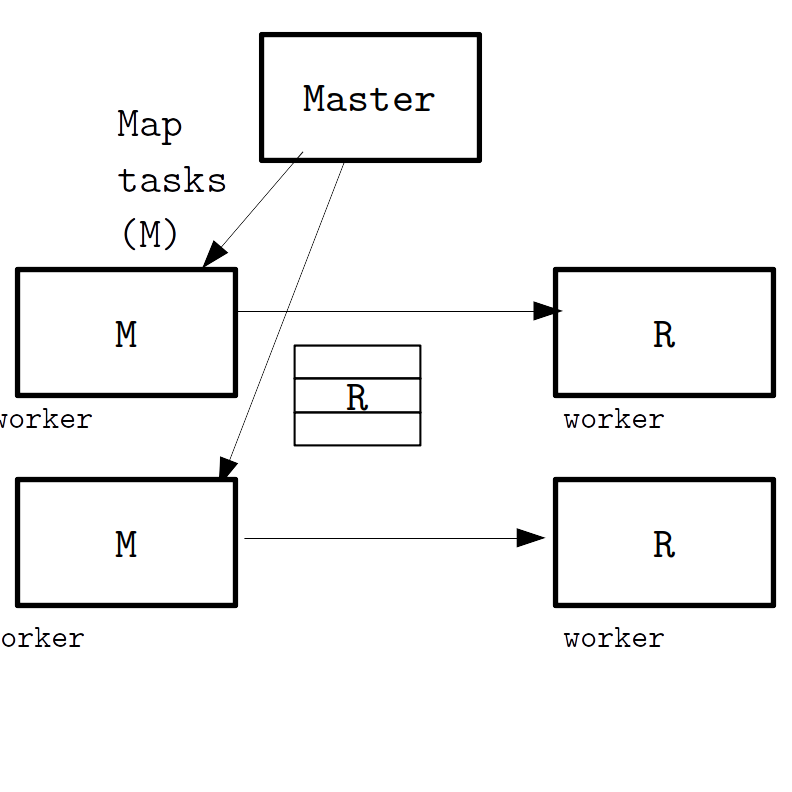
\includegraphics[width=.9\linewidth]{diagrams/masterworker.png}

\subsection{Operators}
\label{sec:orgheadline1}
\begin{enumerate}
\item Map
\begin{itemize}
\item Input = (key,value) --> (key, <v>)
\end{itemize}
\item Reduce
\begin{itemize}
\item Operates share a key
\item (key,value) is sorted and values passed to reducer
\end{itemize}
\end{enumerate}

\subsection{Failures and Slowdowns}
\label{sec:orgheadline3}
\begin{itemize}
\item Handled by the master
\end{itemize}
\subsubsection{Possible failures}
\label{sec:orgheadline2}
\begin{enumerate}
\item Map / Reduce
\begin{itemize}
\item Worker fails, some maps and some reduces completed
\item Reduce data is already written to HDFS, doesn't need to be recomputed
\item Maps must be re-executed to recover intermediate data, since it hasn't been written to HDFS
\end{itemize}
\end{enumerate}

\section{Spark (2.6.19)}
\label{sec:orgheadline8}
\begin{itemize}
\item Programming model
\end{itemize}

\subsection{RDDs}
\label{sec:orgheadline5}
\begin{itemize}
\item Partitioned collection of records
\item SQL, D-Streams, Graphx
\item Intermediate data stored in memory
\item Low overhead fault tolerance achieved through lineage
\end{itemize}

\subsection{Benefits}
\label{sec:orgheadline6}
\begin{enumerate}
\item Speed up iterative computations
\item Load datasets into memory
\begin{itemize}
\item can't be done in MapReduce
\end{itemize}

\item Higher level programs
\end{enumerate}

\Begin{Verbatim}
RDD -> transformations -> action
\end{verbatim}

\begin{itemize}
\item \texttt{Persist} (deserialized, serialized, on-disk)
\begin{itemize}
\item RDDs only exist logically unless \texttt{persist} is called
\begin{itemize}
\item Only then materialized (unless wide dependencies)

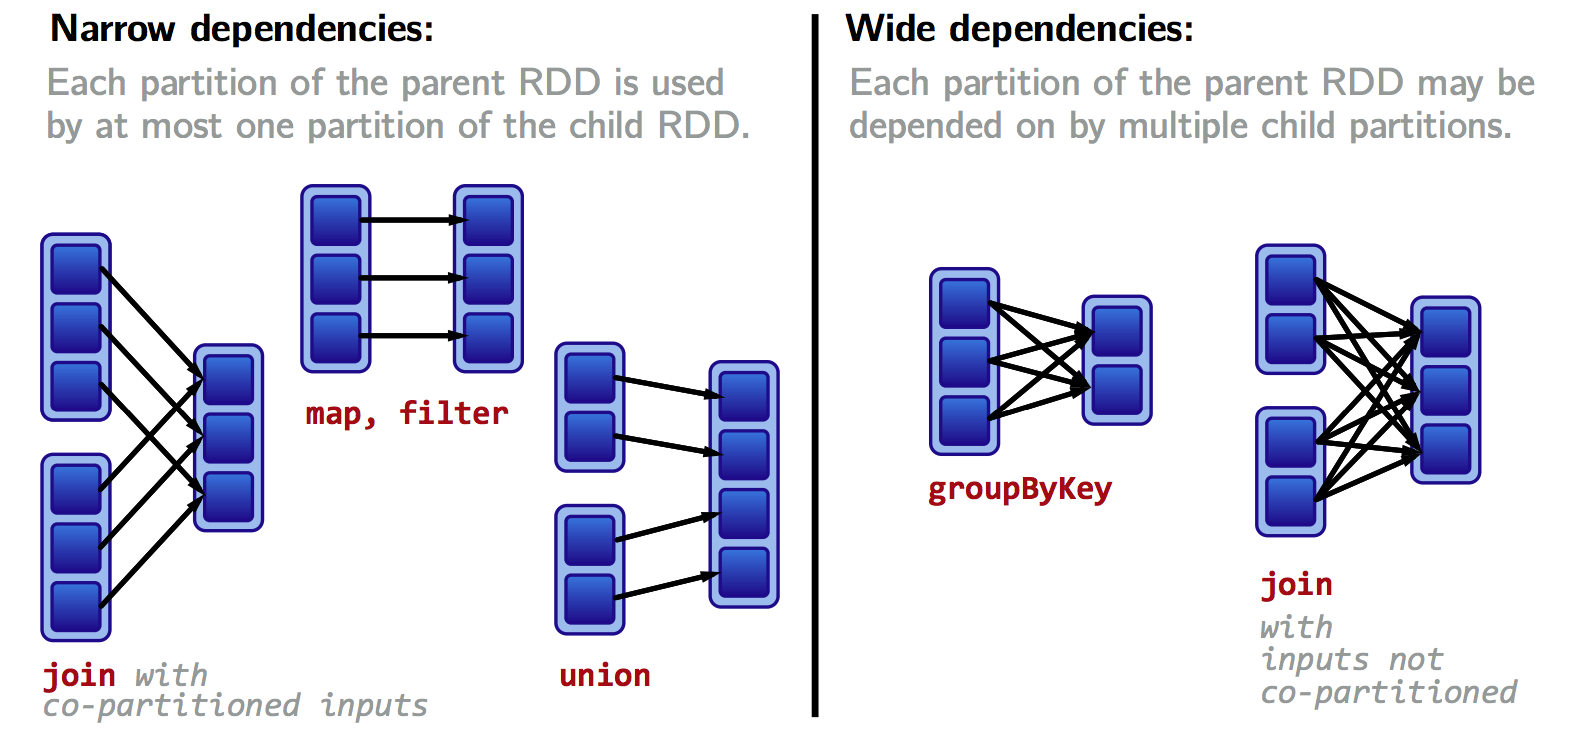
\includegraphics[width=.9\linewidth]{diagrams/widedep.png}
\end{itemize}

\item \texttt{REL} (reliable flag): checkpoint to disk or other memory locations
\end{itemize}
\item Partitioning
\item Lazy computation
\end{itemize}

\subsection{Example: PageRank}
\label{sec:orgheadline7}
\begin{itemize}
\item General process:
\begin{enumerate}
\item Gather
\item Applies
\item Scatter
\end{enumerate}
\end{itemize}

\section{Spark + Job Manager (2.8.19)}
\label{sec:orgheadline11}

\subsection{Job Manager}
\label{sec:orgheadline9}
\begin{itemize}
\item Scheduling: resources, ready, location
\begin{enumerate}
\item How important is the task? (critical path) -> modeling, use some tasks to estimate others
\end{enumerate}
\end{itemize}

\subsection{Stragglers}
\label{sec:orgheadline10}
\begin{enumerate}
\item Rate of progress -> progress report
\begin{itemize}
\item Compare report with model
\item 50\% slower -> this task is a straggler
\item Detect and react to stragglers early
\begin{itemize}
\item No early detection of stragglers in \texttt{MapReduce}
\end{itemize}
\end{itemize}
\item Worthwhile to react to stragglers?
\begin{itemize}
\item Does cloning lower overall resource use?
\end{itemize}
\end{enumerate}

\section{Cluster Schedulers -- Mechanism (2.11.19)}
\label{sec:orgheadline16}

\subsection{Mechanisms}
\label{sec:orgheadline12}
\begin{itemize}
\item YARN: one-level resource allocator
\item Mesos: two-level pessimistic scheduler
\item Omega/Borg: optimistic scheduler

\item Fair allocation - delay scheduling
\end{itemize}

\subsection{YARN}
\label{sec:orgheadline13}
\begin{itemize}
\item Statistical-multiplexing
\begin{itemize}
\item Work-conserving allocation discipline
\begin{itemize}
\item No resources go to waste
\end{itemize}
\end{itemize}
\item \textit{Node Manager (NM)}: local available resources
\item \textit{Resource Manager (RM)}: global state
\item \textit{Application Master (AM)}: requesting for resources
\item De-coupled from programming model
\begin{itemize}
\item Gang scheduling, Message Passing Interface (MPI)
\begin{itemize}
\item Revoking vs. admission control
\end{itemize}
\end{itemize}
\item Late binding (kill-and-restart, e.g.)
\end{itemize}

\subsection{Mesos}
\label{sec:orgheadline15}
\begin{itemize}
\item Two-level scheduler
\item Resource offers
\begin{itemize}
\item Slaves report what resources are available
\item Mesos offers these resources to individual tasks
\begin{itemize}
\item Frameworks can accept or deny offers (maybe they are not data-local)
\end{itemize}
\end{itemize}
\item May kill tasks that run for too long to allow better sharing of resources
\end{itemize}

\subsubsection{Weaknesses}
\label{sec:orgheadline14}
\begin{itemize}
\item Applications cannot request specific resources, must wait until they get offered what they want
\end{itemize}

\section{Omega Scheduler (2.13.19)}
\label{sec:orgheadline18}
\begin{itemize}
\item HFS (delay scheduling)
\item DRF: instantaneous fairness

\begin{enumerate}
\item all-or-nothing
\item priority
\end{enumerate}
\end{itemize}

\subsection{Dominant Resource Fairness}
\label{sec:orgheadline17}
\begin{enumerate}
\item Slots -> rigid
\item Tasks are uniform
\item Equal number of slots is fair
\end{enumerate}
\section{(2.18.19)}
\label{sec:orgheadline23}
\begin{itemize}
\item Resource variabilities (Clarenet, QOOP) | Batch analytics
\item WAN bandwidth -> \textbf{Geo distributed analytics}
\item Compute resources:
\begin{itemize}
\item Spot market
\item Small clusters
\end{itemize}
\end{itemize}

\subsection{Geo Distributed Analytics}
\label{sec:orgheadline22}
\subsubsection{Constraints}
\label{sec:orgheadline19}
\begin{itemize}
\item Bandwidth varies over links (logical link)
\item Control Plane
\begin{itemize}
\item Scheduler
\item Job Manager
\item Parameter server
\item Partitioning/replication/coordination of the above
\end{itemize}
\item Latency
\begin{itemize}
\item Staleness
\item Heartbeats
\end{itemize}
\item Legal \& Privacy Issues
\begin{itemize}
\item Multi-party computation
\end{itemize}
\end{itemize}

\subsubsection{Clarinet}
\label{sec:orgheadline21}
\begin{itemize}
\item Mutually-trusting data centers
\item Batch computation -- multiple queries
\item Ignores legal \& privacy issues
\item Ignores partitioning scheduler or job manager
\end{itemize}
\begin{enumerate}
\item Big ideas
\label{sec:orgheadline20}
\begin{enumerate}
\item Query plans in a network-aware manner
\begin{verbatim}Query => Query Optimizer (n/w aware) => Scheduler =>\end{verbatim}
\begin{itemize}
\item Placement of tasks
\item Scheduling, or "when"
\end{itemize}
\end{enumerate}
\end{enumerate}
\end{document}
